\documentclass[11pt,a4paper]{article}
\usepackage[margin=20mm,headheight=15pt,headsep=7mm,footskip=10mm]{geometry}
\usepackage[T1]{fontenc}
\usepackage{lmodern,amsmath,amssymb,booktabs,tabularx,array,xcolor,enumitem,fancyhdr,microtype,graphicx}
\usepackage{hyperref,xurl}
\definecolor{ink}{HTML}{173445}
\definecolor{teal}{HTML}{146A73}
\definecolor{pale}{HTML}{EDF5F5}
\hypersetup{colorlinks=true,linkcolor=teal,urlcolor=teal,citecolor=teal,pdftitle={Piston pump: concepts, derivations and development roadmap},pdfauthor={MECH0073 PEAR project}}
\setlength{\parindent}{0pt}\setlength{\parskip}{6pt}
\setlength{\abovedisplayskip}{7pt}\setlength{\belowdisplayskip}{7pt}
\setlist[itemize]{leftmargin=5mm,itemsep=3pt,topsep=3pt}
\setlist[enumerate]{leftmargin=6mm,itemsep=3pt,topsep=3pt}
\renewcommand{\arraystretch}{1.16}\setlength{\tabcolsep}{5pt}
\newcolumntype{Y}{>{\raggedright\arraybackslash}X}
\newcolumntype{P}[1]{>{\raggedright\arraybackslash}p{#1}}
\pagestyle{fancy}\fancyhf{}
\fancyhead[L]{\small\sffamily\color{ink}\leftmark}
\fancyhead[R]{\small\sffamily MECH0073 / PEAR}
\fancyfoot[L]{\small Piston pump development record}\fancyfoot[R]{\small\thepage}
\renewcommand{\headrulewidth}{0.3pt}
\newcommand{\chapterpage}[2]{\clearpage\refstepcounter{section}\markboth{\thesection. #1}{}\addcontentsline{toc}{section}{\protect\numberline{\thesection}#1}{\Large\sffamily\bfseries\color{ink}\thesection. #1}\par{\small\color{teal}#2}\par\vspace{2mm}}
\newcommand{\sub}[1]{\par\vspace{1mm}{\large\sffamily\bfseries\color{ink}#1}\par}
\newcommand{\note}[1]{\par\noindent\colorbox{pale}{\parbox{\dimexpr\linewidth-2\fboxsep}{\small #1}}\par}
\newcommand{\dd}{\mathrm d}
\newcommand{\fig}[3]{\begin{center}\includegraphics[width=\linewidth,height=#2,keepaspectratio]{assets/#1}\end{center}{\small\textbf{Figure.} #3}\par}
\numberwithin{equation}{section}
\begin{document}
\thispagestyle{empty}
{\large\sffamily\color{teal}MECH0073 / EXPERIMENTAL EVAR RIG}\par\vspace{12mm}
{\Huge\sffamily\bfseries\color{ink}Piston pump}\par
{\LARGE\sffamily Concepts, derivations and development roadmap}\par\vspace{6mm}
{\large Team review / 23 November 2026}\par\vspace{8mm}
\note{\textbf{Current position:} a literature-informed analytical framework, original concept sketches and separately executed reference calculations. The current enforced-valve design is not yet one verified coupled simulation. No final geometry, architecture or maximum drive-force rating has been selected.}
\vspace{5mm}
\sub{The question we are trying to answer}
How do piston geometry, motion, retained air, valve coordination and the connected circuit determine delivered flow, pressure waveforms and hydraulic force? Use that relationship to choose a feasible pump for controlled EVAR benchtop experiments, then develop the interactive MATLAB model.
\sub{Starting operating point}
\begin{center}\Large
\textbf{5 L/min}\quad at\quad\textbf{75 pulses/min}\par
\normalsize per arterial circuit; required net delivery approximately \textbf{66.7 mL/pulse}.
\end{center}
\sub{How to use this report}
The opening pages provide the team summary, qualitative advantages and limitations, and all three supplied concept images. The technical record then develops the mathematics from geometry to circuit loading and valve coordination. Existing numerical examples retain their original assumptions. The final pages set out decisions, completion gates, measurement needs and traceability.
\textbf{Reading convention.} A requirement is prescribed; a trial input is assumed; a calculated result follows from a stated model; a verified calculation is not a physically validated pump. Gas pressures use absolute pressure. Other pressures use a common gauge reference unless stated otherwise.
\vfill
{\small This is a consolidated record of work to date. The full-liquid limit and passive-valve model are retained as analytical comparators. The selected direction uses enforced valves, adjustable timing and an explicit dry-side pressure boundary. The mechanism comparison is qualitative, with no scores or ranking.}

\clearpage\markboth{Contents}{}{\small\setlength{\parskip}{0pt}\tableofcontents}

\chapterpage{Team summary}{Purpose, completed work and current limits}
We are developing a reciprocating flat-face plunger pump to create controlled pulsatile boundary conditions in the EVAR rig. Both a shared chamber alternating between ventricular duties and two dedicated ventricular chambers remain under consideration. The pump must operate with the reservoirs, Windkessels, phantom and sensors; their interaction determines the resulting waveform.
\sub{Work completed}
\begin{itemize}
\item Established the baseline delivery requirement: $5000/75=66.67$ mL per circuit pulse, with a period of $0.8$ s.
\item Reviewed cardiovascular piston-pump literature, separating pumps used as mock ventricles, waveform generators, hydraulic actuators and tissue-conditioning devices. An LVAD under test is not the same component as the rig pump.
\item Derived geometry, conservation, waveform scaling, open-path losses and inertia, external-load response, retained-air compliance, valve eligibility and pressure-force relationships.
\item Executed separate Python reference studies for gas/passive-valve behaviour, waveform candidates and prescribed-flow arterial loads; developed a formula-based spreadsheet.
\item Recorded the variable register, assumptions, decisions, operating budgets and verification scope in the design branch.
\item Made the dry-side boundary explicit: a closed rear chamber can change pressure with displacement and may have an effective area different from the wetted face.
\end{itemize}
\sub{What this enables now}
The framework explains why changes in diameter, stroke, pulse rate, valve area and timing have coupled consequences. It identifies which quantities require measurement and which calculations are valid only in a restricted limit. It supports a structured next derivation and avoids choosing geometry from an isolated mean-flow or pressure value.
\sub{What is not yet established}
We do not yet have a verified whole-cycle solution combining the current enforced valve law, retained air, dynamic circuit load, rear pressure and either complete architecture. The spreadsheet and existing Python studies are useful components, not interchangeable versions of that final model. MATLAB files have been statically checked previously, but the current numerical model has not been run in MATLAB. No prototype performance or clinical predictive validity is established.
\note{\textbf{Immediate milestone:} one explicitly defined chamber with its circuit load, a consistent ideal-valve treatment, and verified pressure, flow, liquid inventory and hydraulic-force histories.}

\chapterpage{Why consider a piston mechanism?}{Qualitative benefits and limitations; no ranking}
Published piston systems have generated physiological flow profiles for aortic experiments \cite{chaudhury,franzetti}. This establishes a useful precedent, not the performance of our proposed assembly. The following trade-offs are engineering implications of our present model.
\sub{Advantages}
\begin{itemize}
\item \textbf{Direct displacement relationship.} Bore and travel give a transparent geometric volume; measured position can be linked to commanded displacement.
\item \textbf{Pulsatile operation.} Filling and delivery strokes provide a natural means of creating distinct flow phases.
\item \textbf{Adjustable waveform potential.} An appropriate actuator can change the speed profile and timing without changing the basic chamber arrangement.
\item \textbf{Interpretable design choices.} Larger bore reduces travel at a given sweep; smaller bore reduces pressure force at a given chamber pressure, with greater travel required.
\item \textbf{Observable behaviour.} Pressure, flow and position provide direct measurements against which to check the hydraulic model and later develop feedback.
\end{itemize}
\sub{Limitations and engineering costs}
\begin{itemize}
\item \textbf{Fixed stroke couples flow and rate.} Independent selection needs an additional means of changing net delivery.
\item \textbf{Sweep is not measured delivery.} Gas storage, underfilling, valve behaviour, leakage or diversion can change the outlet integral.
\item \textbf{Pressure is a circuit response.} Geometry and motion cannot independently impose any desired pressure and flow on an unchanged passive load.
\item \textbf{Valve coordination matters.} Switching influences inventory, filling and pressure. Ideal closure does not establish the real transient peak.
\item \textbf{Motion flexibility is conditional.} A constant-speed fixed crank constrains the waveform. Arbitrary motion requires suitable actuation or transmission.
\item \textbf{Mechanical loads remain to be completed.} Seals, friction, moving-solid inertia, rear pressure and converter geometry affect the eventual drive requirement. No low-cost, low-noise or low-maintenance claim is established yet.
\end{itemize}
\sub{Architecture trade-off}
\par
\begin{tabularx}{\linewidth}{@{}P{.22\linewidth}YY@{}}\toprule
Concept & Potential benefit & Main complication\\\midrule
1A: shared chamber & One piston assembly performs both duties. & Routing between different pressure circuits; shorter duty budgets; state carry-over.\\
1B: two chambers & Separate pulmonary/systemic roles and overlapping cycles. & Additional hardware and coordinated valves; sustained circuit balance.\\\bottomrule
\end{tabularx}\par

\chapterpage{Original sketches: opposed chambers}{Supplied images reproduced without redrawing or inferred geometry}
\fig{early_pump_schematic.png}{61mm}{Early pump schematic supplied in the conversation. It illustrates one side discharging while the opposite side fills. Its original source beyond the supplied upload is not established.}
\fig{early_opposed_sketch.jpeg}{119mm}{Original handwritten valve/chamber mapping. Labels and dimension symbols are preserved as drawn; they are not selected dimensions.}
\textbf{Interpretation.} For a common separating piston in fixed end chambers, advance reduces one volume while increasing the other. That opposes their filling/ejection phases. The later two-piston concept was introduced to allow both ventricular duties to contract together or with a chosen offset. This early image remains concept history; the apparent wet rod in a schematic does not override the subsequent flat wetted-face requirement.

\chapterpage{Original sketch: concept development}{Shared state-dependent chamber and two dedicated chambers}
\begin{center}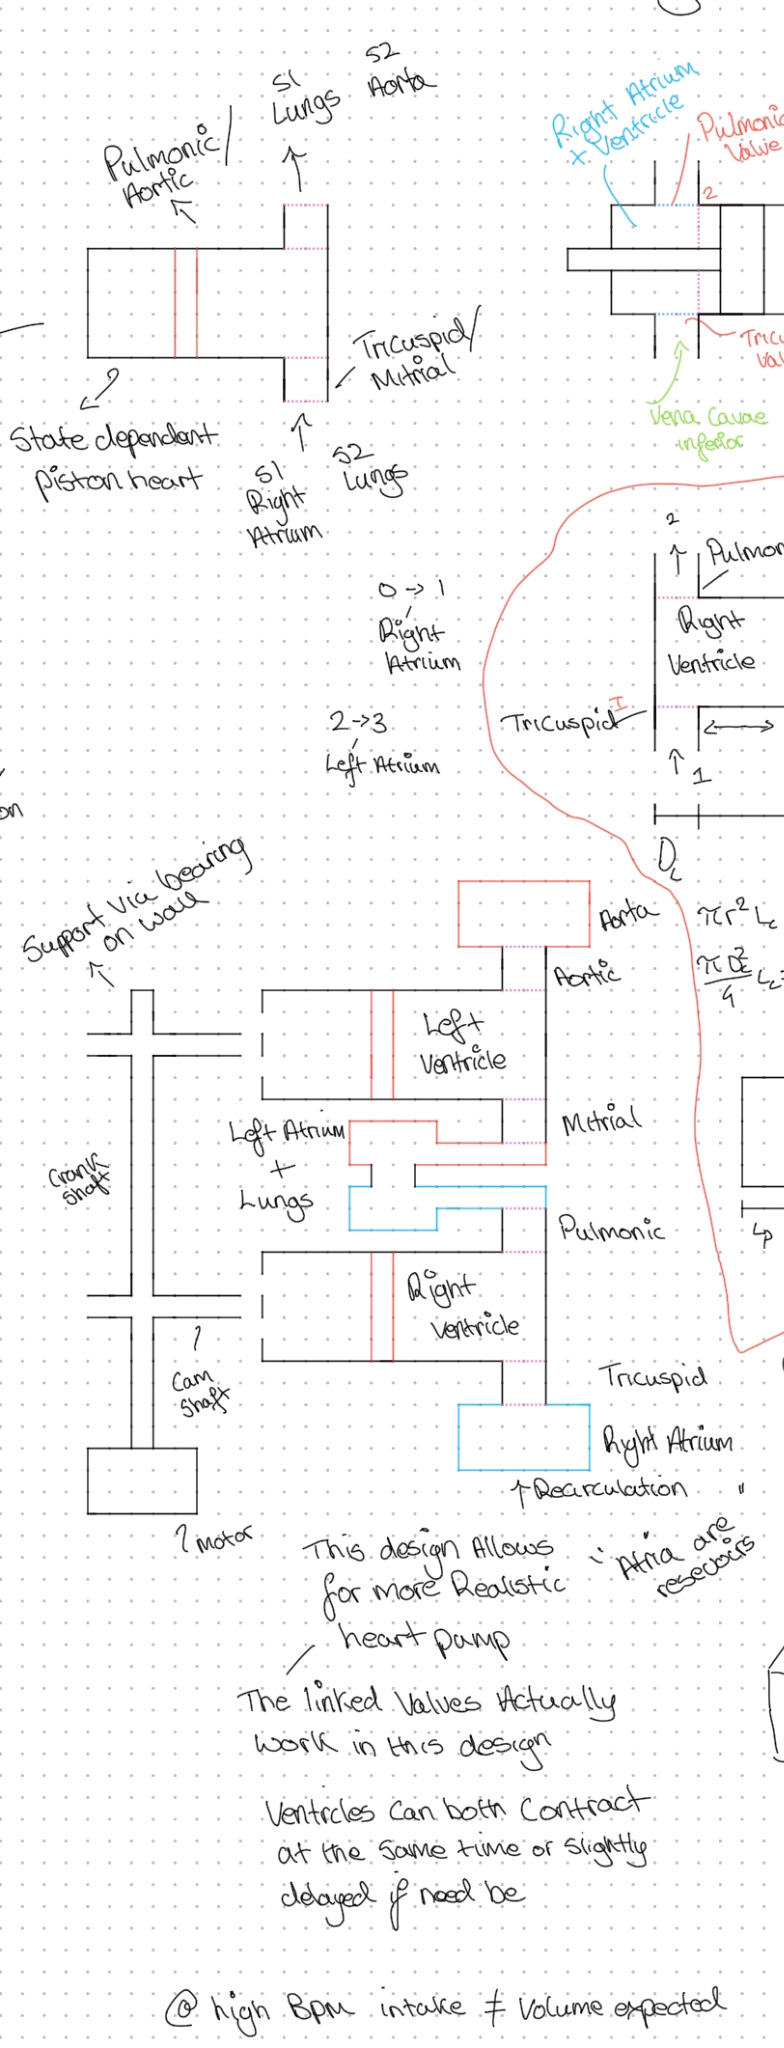
\includegraphics[height=205mm,width=\linewidth,keepaspectratio]{assets/concept_development.jpeg}\end{center}
{\small \textbf{Figure.} Original concept sheet supplied on 21 November 2026. The upper-left sketch assigns a shared chamber different duties; the lower sketch shows two chambers and reservoir connections with an illustrative mechanical translator. The supplied image is cropped at the right edge; missing geometry is not reconstructed. Crank/cam details remain concept proposals, not selected kinematics.}

\clearpage\markboth{Concept sketch: enlarged excerpts}{}
\phantomsection\addcontentsline{toc}{subsection}{Concept sketch: enlarged excerpts}
{\Large\sffamily\bfseries\color{ink}Concept sketch: enlarged excerpts}\par
{\small\color{teal}Details from the full original on the preceding page; no geometry added}\par
\sub{Shared chamber with assigned duties}
\begin{center}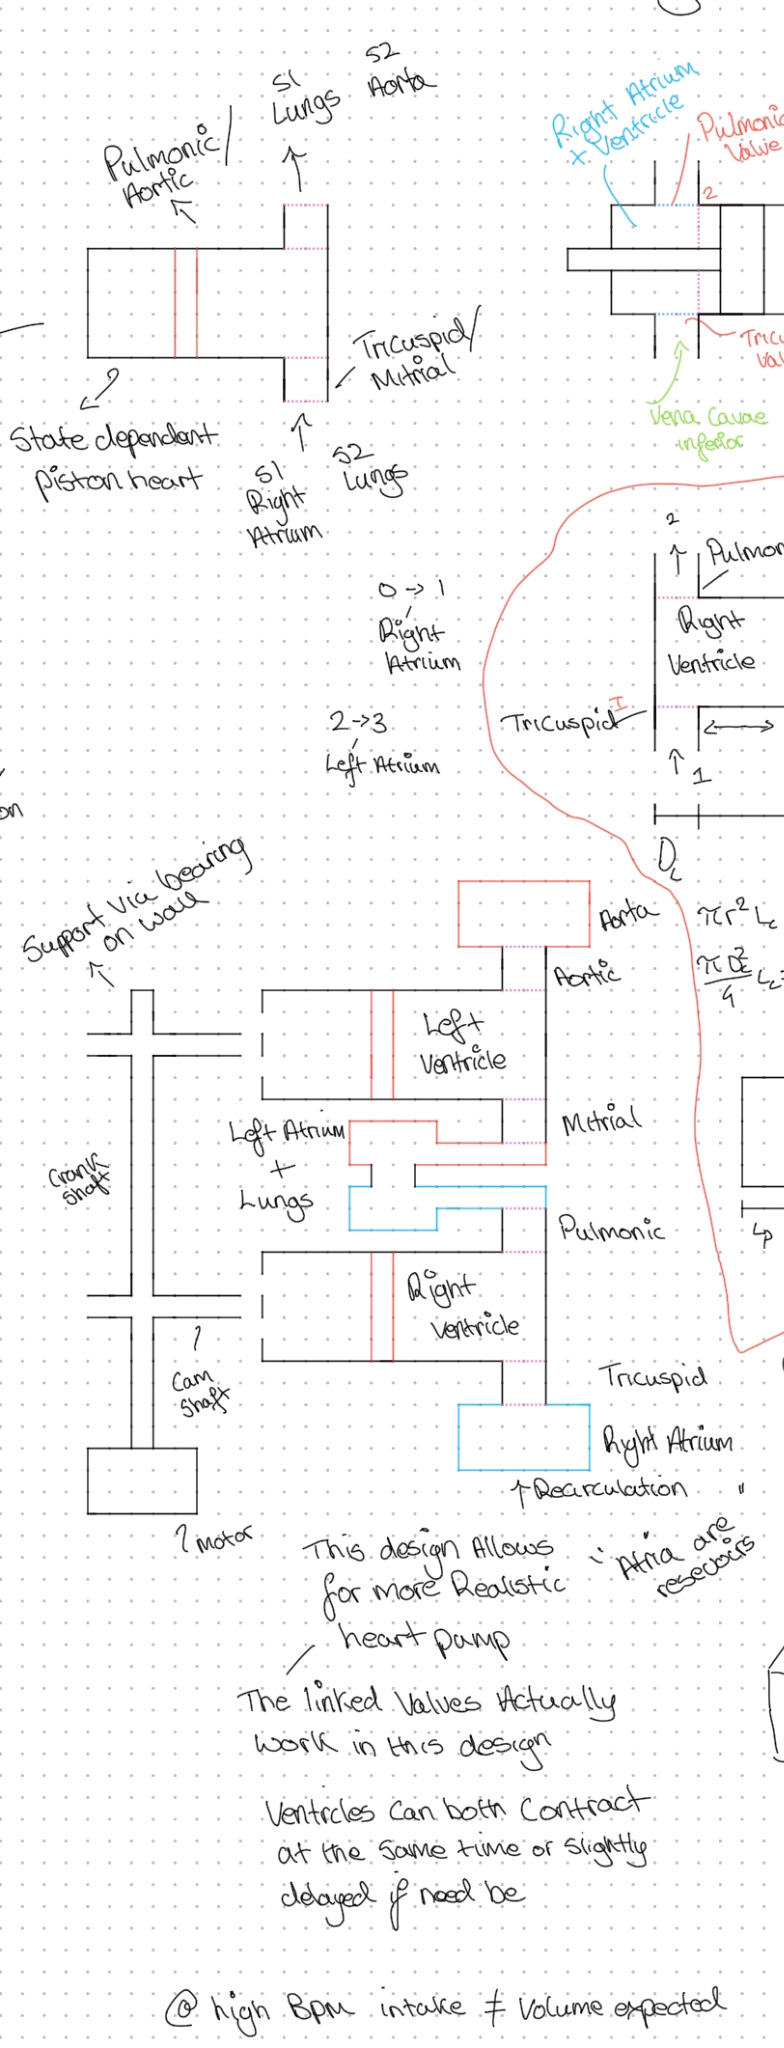
\includegraphics[width=.88\linewidth,height=65mm,keepaspectratio,trim={0bp 1448bp 224bp 0bp},clip]{assets/concept_development.jpeg}\end{center}
{\small The same chamber alternates its inlet/outlet circuit assignments. Selector transitions and hydraulic state carry-over remain to be modelled.}\par
\sub{Two dedicated chambers and reservoirs}
\begin{center}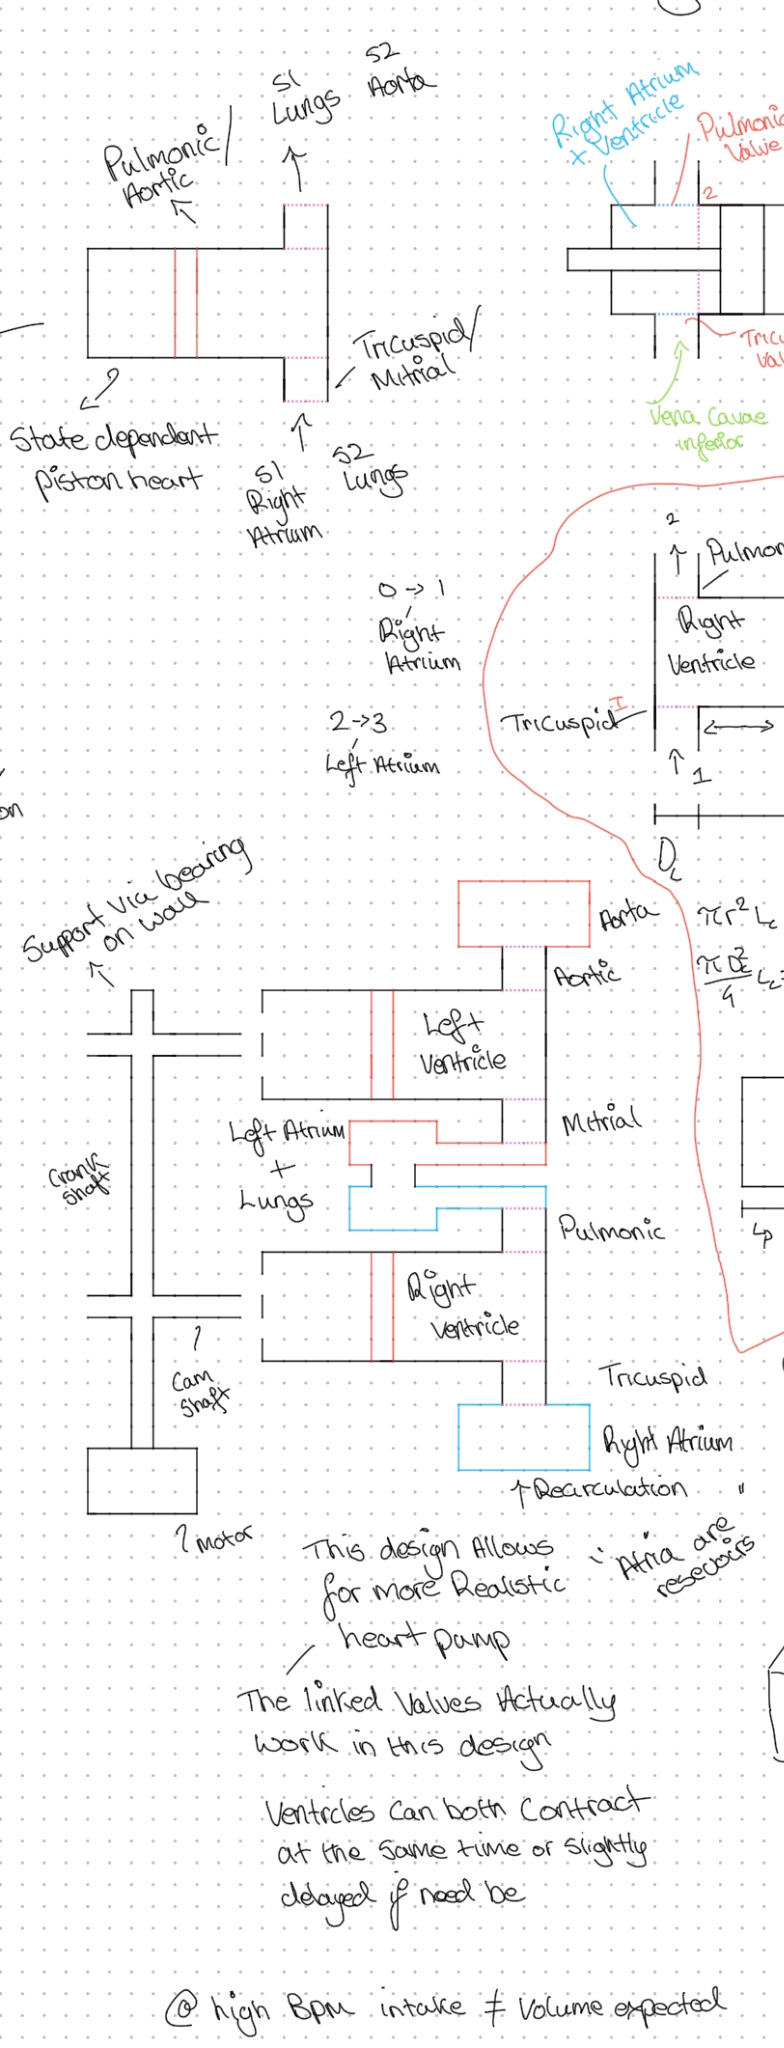
\includegraphics[width=.94\linewidth,height=108mm,keepaspectratio,trim={0bp 418bp 0bp 810bp},clip]{assets/concept_development.jpeg}\end{center}
{\small Separate ventricular chambers permit overlapping cycles. The drawn shaft/cam arrangement is a concept for actuation, not a completed mechanism design.}\par

\chapterpage{System definition and notation}{One chamber first; two architectures built from the same hydraulic block}
The inlet path runs from an atrial reservoir to the chamber; the outlet path runs from the chamber to an arterial load. Define pressure stations before assigning losses. The phantom lies downstream in its actual circuit, so pump-outlet signals are not automatically phantom-inlet signals.
\par
\begin{tabularx}{\linewidth}{@{}P{.22\linewidth}Y P{.19\linewidth}@{}}\toprule
Symbol & Meaning & SI unit\\\midrule
$D_p,A_p,S,x$ & Wetted diameter, area, travel and advance from full retraction & m, m$^2$, m, m\\
$v,a$ & $\dot x,\ddot x$: piston speed and acceleration & m/s, m/s$^2$\\
$V_c,V_\ell,V_g$ & Total chamber, liquid and retained front-gas volume & m$^3$\\
$Q_p,Q_i,Q_o$ & Displacement rate; inlet and outlet liquid flow & m$^3$/s\\
$p_i,p_c,p_a,p_b$ & Inlet, chamber, arterial/load inlet and dry-rear pressure & Pa gauge\\
$P_g,P_b,p_{\rm atm}$ & Front/rear absolute gas and ambient pressure & Pa absolute\\
$p_w,p_r$ & Windkessel compliance-node and return pressure & Pa gauge\\
$R,B,I$ & Linear loss, quadratic loss and fluid inertance & Pa s/m$^3$, Pa s$^2$/m$^6$, Pa s$^2$/m$^3$\\
$C_g,C_W,C_{\rm wall}$ & Front gas, external load and chamber-wall compliance & m$^3$/Pa\\
$h,f,T_H$ & Per-circuit pulse rate, chamber event rate, circuit period & min$^{-1}$, min$^{-1}$, s\\
$\lambda_R,\gamma_d$ & Shared right-duty fraction; within-duty advance fraction & dimensionless\\
$u_j,a_j$ & Valve command and effective opening fraction & dimensionless\\
$A_b,V_b,n_b$ & Effective rear area, gas volume, polytropic exponent & m$^2$, m$^3$, dimensionless\\\bottomrule
\end{tabularx}\par
\sub{Conventions and initial assumptions}
$x$ increases into the wet chamber. $Q_i>0$ enters it; $Q_o>0$ leaves it. Commanded open paths can carry signed flow unless one-way behaviour is separately specified. Neglect external leakage initially. Use a rigid chamber and incompressible liquid for the gas-pocket model, approximately uniform piston-face pressure, and the same pressure datum throughout.
\begin{equation}
1\ \mathrm{mL}=10^{-6}\ \mathrm{m^3},\quad
1\ \mathrm{L/min}=\frac{1}{60000}\ \mathrm{m^3/s},\quad
1\ \mathrm{mmHg}\simeq133.322\ \mathrm{Pa}.
\end{equation}
The notation $C_W$ here always means external Windkessel compliance; $C_{\rm wall}$ means chamber-wall compliance. Earlier notes used overlapping subscripts, which are separated here. The full typed variable register remains in \path{VARIABLES.csv}.

\chapterpage{Geometry, volume and mean flow}{Foundational derivation and the fixed-stroke constraint}
For the flat wetted face, with no wetted-rod deduction,
\begin{equation}
A_p=\frac{\pi D_p^2}{4},\qquad V_s=A_pS,\qquad
V_c(x)=V_{c0}-A_px,\qquad \dot V_c=-A_p\dot x.
\end{equation}
$V_{c0}$ includes chamber-side residual/dead volume at full retraction. For a simple internal piston geometry only,
\begin{equation}
S_{\rm available}=L_{\rm internal}-t_p-c_{\rm front}-c_{\rm rear}.
\end{equation}
$t_p$ is piston thickness and $c$ denotes end clearance. Ports, seals and mechanical limits can further restrict travel. Therefore $S=L-t_p$ is not a general construction rule.

For incompressible liquid, no gas and no leakage,
\begin{equation}
\frac{\dd(\rho V_c)}{\dd t}=\rho Q_i-\rho Q_o
\quad\Longrightarrow\quad Q_o-Q_i=A_p\dot x=Q_p.
\end{equation}
An isolated ejection phase gives $Q_o=A_p\dot x$; isolated filling gives $Q_i=-A_p\dot x$. Both valves closed require $\dot x=0$ in this rigid, incompressible limit. Integrating a complete isolated advance gives $V_{\rm net}=A_pS$ only under these assumptions.

More generally, let $T$ be the complete cycle period in seconds; use signed outlet flow and the actual measurement boundary:
\begin{equation}
V_{\rm net}=\int_{\rm cycle}Q_o\,\dd t,\qquad
\overline Q=\frac{V_{\rm net}}{T},\qquad
\eta_d\equiv\frac{V_{\rm net}}{V_s}.
\end{equation}
For one delivery per circuit pulse, in display units,
\begin{equation}
\overline Q[\mathrm{L/min}]=\frac{hV_{\rm net}[\mathrm{mL}]}{1000},\qquad
V_{\rm net,target}=\frac{1000\overline Q_{\rm target}}h.
\end{equation}
At 5 L/min and 75/min, the target is $66.667$ mL/pulse. An \emph{illustrative} $D_p=50$ mm gives $S=33.953$ mm for that ideal geometric sweep. No bore has been selected.
\begin{equation}
S=\frac{4V_s}{\pi D_p^2},\qquad
A_p=\frac{\overline Q T}{\eta_d S}\quad\text{with SI units throughout}.
\end{equation}
Frequency has not disappeared: it is embedded in the required per-event volume. $A_p=V_s/S$ is merely the geometry expression. The delivery ratio is a calculated diagnostic, not an independent control input or necessarily a conventional efficiency bounded by one when through-flow is permitted.
\note{Advance and return must have equal net travel over a repeating cycle. Their durations, speeds and accelerations can differ; unequal net travel would cause positional drift.}

\chapterpage{Operating strategies and adjustable timing}{Separate pulse rate, duty allocation and actual delivery duration}
Keep both strategies open: fixed stroke with flow allowed to rise with rate, or fixed stroke with an added means of changing net delivery. For the illustrative $66.667$ mL sweep:
\begin{center}\begin{tabular}{@{}rrrr@{}}\toprule
$h$ (/min)&Ideal flow (L/min)&Volume for 5 L/min (mL)&Ideal diversion\\\midrule
40&2.667&125.00&Insufficient sweep\\75&5.000&66.67&0\%\\120&8.000&41.67&37.5\%\\180&12.000&27.78&58.3\%\\\bottomrule
\end{tabular}\end{center}
Diversion, controlled inlet spill, variable travel or exchangeable geometry are possible approaches to investigate, not implemented choices. Skipping deliveries changes actual pulse frequency. Neither passive storage nor uncontrolled underfilling independently commands mean flow.

For per-circuit rate $h$, define $T_H=60/h$. Each dedicated chamber in 1B has the full $T_H$; cycles may overlap. For 1A,
\begin{equation}
T_R=\lambda_RT_H,\quad T_L=(1-\lambda_R)T_H,\quad0<\lambda_R<1.
\end{equation}
The default $\lambda_R=0.5$ gives two 0.4 s duties at 75/min. With $\lambda_R=0.6$, the budgets are 0.48 s right and 0.32 s left. The mean event count remains $2h$, but unequal slots are not uniformly spaced cycles at $2h$.
With $s=(t-t_0)\bmod T_H$,
\begin{equation}
x(t)=\begin{cases}S X_R(s/T_R),&0\le s<T_R,\\
S X_L((s-T_R)/T_L),&T_R\le s<T_H.\end{cases}
\end{equation}
Each $X_d$ is a complete advance/return waveform with compatible endpoint derivatives. Within duty $d$, in the no-dwell illustration,
\begin{equation}
t_{e,d}=\gamma_dT_d,\quad t_{f,d}=(1-\gamma_d)T_d,\quad
r_d=\frac{t_{e,d}}{t_{f,d}},\quad\gamma_d=\frac{r_d}{1+r_d}.
\end{equation}
The provisional 60:40 means \textbf{return:advance}, initially $\gamma_d=0.4$. For the full-liquid isolated phases it also represents filling:ejection. With gas/valves, actual flow durations can differ. Routing or dwell must fit within the budget, not be silently added.
\begin{equation}
\dot x\propto S/T_d,\quad\ddot x\propto S/T_d^2.
\end{equation}
At fixed sweep and time-scaled shape, flow scales with rate; quadratic loss and inertial pressure scale with rate squared. Increasing 75 to 180/min gives factors 2.4 and 5.76 respectively, under those assumptions. Physiological right/left timing can differ \cite{leighton,hirschfeld}; the shared duty split is an engineering allocation, not an anatomical half-cycle.

\chapterpage{Waveform families}{Normalise shape and timing to the required phase volume}
For dimensionless phase time $u\in[0,1]$, positive shape $g_j$ and phase duration $t_j$,
\begin{equation}
G_j=\int_0^1g_j(u)\,\dd u,\quad
\phi_j=\frac{g_j}{G_j},\quad Q_j(t)=\frac{V_s}{t_j}\phi_j(u).
\end{equation}
This gives $\int Q_j\dd t=V_s$. A selected shape, duration and phase volume fix peak flow; it is not a fourth independent input.
\sub{Half-sine reference}
\begin{equation}
g(u)=\sin(\pi u),\quad G=2/\pi,\quad
Q_e=\frac{\pi V_s}{2t_e}\sin(\pi t/t_e).
\end{equation}
\sub{Historical harmonic templates}
The following coefficients were previously inspected in the supplied Franzetti article, Eqs. 14--15 \cite{franzetti}, which attributes them to Swanson--Clark and Talukder--Reul. The original 1977/1978 papers were not independently inspected.
\begin{align}
g_e(u)&=0.924\sin(\pi u)+0.230\sin(2\pi u)+0.092\sin(3\pi u),\\
G_e&=\frac2\pi\left(0.924+\frac{0.092}{3}\right),\\
g_f(u)&=0.520\sin(\pi u)+0.257\sin(2\pi u)+0.479\sin(3\pi u),\\
G_f&=\frac2\pi\left(0.520+\frac{0.479}{3}\right).
\end{align}
Our separate phase normalisation is not the paper's complete optimisation routine. It retains the template shape while enforcing equal phase volumes.
\sub{Quintic position reference}
\begin{equation}
H(u)=10u^3-15u^4+6u^5,\quad H'(u)=30u^2(1-u)^2.
\end{equation}
Use $x=SH(t/t_e)$ on advance and $x=S[1-H((t-t_e)/t_f)]$ on return. Endpoint speed and acceleration vanish for any positive durations. This is an engineering smoothness reference, not a physiological prescription.

For each normalised pair,
\begin{equation}
Q_p=\begin{cases}(V_s/t_e)\phi_e(t/t_e),&0\le t\le t_e,\\
-(V_s/t_f)\phi_f((t-t_e)/t_f),&t_e<t\le T.\end{cases}
\end{equation}
Negative displacement flow represents retraction; it does not itself command reverse flow at the aortic outlet. Other literature candidates include segmented cosine volume commands and measured traces, but they have not been implemented in these comparisons.

\chapterpage{Smooth joining without changing volume}{Derivation 02: our engineering extension}
Raw half-sine and harmonic flow shapes vanish at their endpoints, but their slopes generally do not. Unequal phase durations can therefore produce acceleration jumps even when position and velocity are continuous.
For endpoint fraction $0<\epsilon\le0.5$, use
\begin{equation}
w_\epsilon(u)=\begin{cases}
H(u/\epsilon),&0\le u<\epsilon,\\
1,&\epsilon\le u\le1-\epsilon,\\
H((1-u)/\epsilon),&1-\epsilon<u\le1,
\end{cases}
\end{equation}
where $H$ is the quintic above. At $\epsilon=0$, use $w=1$ as a separate unsmoothed case.
\begin{equation}
G_j=\int_0^1g_jw_\epsilon\,\dd u,\quad
\phi_j=\frac{g_jw_\epsilon}{G_j},\quad
Q_p=\sigma_j\frac{V_s}{t_j}\phi_j,\quad\sigma_e=1,\ \sigma_f=-1.
\end{equation}
Differentiate with $\dot u=1/t_j$:
\begin{equation}
\dot Q_p=\sigma_j\frac{V_s}{t_j^2}
\frac{g'_jw_\epsilon+g_jw'_\epsilon}{G_j},\qquad
\dot x=\frac{Q_p}{A_p},\quad\ddot x=\frac{\dot Q_p}{A_p}.
\end{equation}
Integrating gives the position command:
\begin{equation}
\frac{x}{S}=\begin{cases}\int_0^u\phi_e(v)\,\dd v,&\text{advance},\\
1-\int_0^u\phi_f(v)\,\dd v,&\text{return}.\end{cases}
\end{equation}
With positive $\epsilon$, flow and its first two derivatives vanish at phase endpoints. This provides smooth motion joins, but does not resolve hydraulic pressure switching. The workbook used 400 trapezoidal intervals per phase; Python checked quadrature against high-order integration and derivative/endpoint conditions.

\begin{center}\small\begin{tabular}{@{}lrrrr@{}}\toprule
Shape pair & $\epsilon$ & Peak $Q_e$ & Peak $Q_i$ & Max $|\ddot x|$\\
& & L/min & L/min & m/s$^2$\\\midrule
Half-sine & 0 &19.635&13.090&1.636\\
Half-sine &0.05&19.704&13.136&2.909\\
Harmonics &0&20.567&19.401&2.845\\
Harmonics &0.05&20.658&19.598&5.026\\\bottomrule
\end{tabular}\end{center}
These are existing kinematic calculations at 5 L/min, 75/min, $\gamma=0.4$, $D_p=50$ mm. Smoothing removes jumps but increases the finite acceleration peak by approximately 77--78\% here. No smoothing width or force improvement is selected.

\chapterpage{Existing waveform comparisons}{Prescribed commands; actual gas-coupled outlet flow remains to be solved}
\fig{waveforms.png}{104mm}{Raw normalised waveform study: half-sine, harmonic and quintic references. Each ideal phase encloses 66.67 mL.}
\fig{waveform_smoothing.png}{104mm}{Existing endpoint-smoothing comparison. Smooth motion does not by itself prove continuous or physiological chamber pressure. Figures are reproduced from stored calculations; no new pump simulation was run for this report.}

\chapterpage{Open-path pressure from momentum and losses}{Derivation 01: one inlet or outlet branch}
For a uniform liquid column, $m=\rho A_tL$ and mean speed $U=Q/A_t$. Newton's law gives
\begin{equation}
m\dot U=\rho L\dot Q,\qquad
\Delta p_{\rm inertia}=\frac{\rho L}{A_t}\dot Q=I\dot Q.
\end{equation}
Inertance stores and returns kinetic energy; its pressure contribution changes sign during deceleration. A provisional open-branch law is
\begin{equation}
\boxed{p_{\rm up}-p_{\rm down}=RQ+BQ|Q|+I\dot Q.}
\end{equation}
Assume pressure stations have the same elevation and unresolved velocity-head differences are negligible. Otherwise add hydrostatic and reversible kinetic-pressure terms separately. Do not describe pressure recovery as dissipative loss.
\begin{align}
R_{\rm lam}&=\frac{128\mu L}{\pi D_t^4},& A_t&=\frac{\pi D_t^2}{4},\\
B_v&=\frac{\rho}{2(C_dA_v)^2},& B_{\rm local}&=\frac{\rho K}{2A_t^2},\\
I&=\frac{\rho L}{A_t}.&&
\end{align}
$\mu$ is dynamic viscosity (Pa s), $\rho$ density (kg/m$^3$), $C_d$ discharge coefficient and $K$ a local loss coefficient. $A_v$ is effective valve area, not necessarily nominal connection area. The laminar expression requires a fully developed Newtonian reference flow; it is not an established friction law for all pulsatile BMF conditions.

The valve term follows from $Q=C_dA_v\sqrt{2\Delta p/\rho}$ for forward quasi-steady flow. At fixed $Q,C_d$ and circular effective opening, $\Delta p_v\propto d_v^{-4}$. At fixed available pressure, a larger opening instead allows more flow. These are different boundary-condition comparisons.
\sub{Tapered passage correction retained from the literature audit}
For a slowly varying circular passage treated as local Poiseuille elements, $D(z)=D_{\rm in}+(D_{\rm out}-D_{\rm in})z/L$:
\begin{equation}
R=\frac{128\mu}{\pi}\int_0^L\frac{\dd z}{D(z)^4}
=\frac{128\mu L}{3\pi(D_{\rm in}-D_{\rm out})}
\left(D_{\rm out}^{-3}-D_{\rm in}^{-3}\right).
\end{equation}
The equal-diameter limit recovers $128\mu L/(\pi D^4)$. The printed thesis expression appeared to omit the factor $1/3$ \cite{thesis}; stored numerical integration agreed with this corrected expression. This concerns the printed equation, not uninspected original code. Losses fitted as a combined component curve must not be counted again through separate $R$ or $B$ terms.

\chapterpage{Full-liquid phase pressures and geometry effects}{Conditional equations; switching is outside this limiting calculation}
Define $\Delta p_i=p_i-p_c$ and $\Delta p_o=p_c-p_a$, with separate inlet/outlet coefficients. In ejection with the inlet closed,
\begin{equation}
Q_o=A_pv,\quad\dot Q_o=A_pa,\quad
p_c=p_a+R_oA_pv+B_o(A_pv)^2+I_oA_pa.
\end{equation}
In filling with the outlet closed,
\begin{equation}
Q_i=-A_pv,\qquad
p_c=p_i-R_iQ_i-B_iQ_i^2-I_i\dot Q_i.
\end{equation}
Filling pressure can fall below reservoir pressure during acceleration. During deceleration the inertial contribution reverses sign. These phase expressions do not guarantee that a passive valve would remain in the assumed state; an enforced closure has a different rule.

For the general rear-area force balance developed later, with a common gauge reference,
\begin{align}
F_h&=A_pp_c-A_bp_b,\\
F_h&=A_pp_a-A_bp_b+R_oA_p^2v+B_oA_p^3v^2+I_oA_p^2a
\quad\text{(ejection)}.
\end{align}
The earlier $A_p(p_c-p_b)$ form is recovered only when $A_b=A_p$. Each term is a force in N. Hydraulic inertia already included in $p_c$ must not be added again.
\sub{Changing piston size while holding the delivery waveform fixed}
With fixed required volume and the same $Q_p(t)$, increasing area reduces stroke, speed and acceleration in inverse proportion to $A_p$. With unchanged fluid paths, the calculated pressure is unchanged in this full-liquid approximation; hydraulic force grows with area. Doubling bore therefore quarters travel and quadruples force if both pressure exposures/area ratios are otherwise unchanged. Holding travel fixed instead is a different experiment because it increases swept volume.
\sub{Why smooth reversals did not complete the pressure model}
At a zero-flow, zero-flow-acceleration ejection endpoint, this phase law gives $p_c=p_a$. At the start of filling it gives $p_c=p_i$. When those pressures differ, simply joining the phases produces an unexplained pressure jump. Finite chamber storage and a consistent valve sequence are required.
\note{Full retraction fixes position and total geometric volume, not pressure or maximum force. Gas state, valve state, flow acceleration and rear pressure must also be known. A settled open-port dwell is only a special case.}

\chapterpage{External load and periodic pressure solution}{Derivation 03: Windkessel interface without designing its hardware}
For a three-element arterial load,
\begin{equation}
p_a=p_w+R_1Q_o,\qquad
C_W\dot p_w=Q_o-\frac{p_w-p_r}{R_2}.
\end{equation}
$R_1,R_2$ are distinct load resistances, $C_W$ is load compliance, and $p_r$ is terminal return pressure. The inlet-reservoir pressure $p_i$ is distinct from $p_r$ and rear pressure $p_b$. These equations determine $p_a$ when $Q_o$ is known; do not also impose an independent $p_a(t)$.
Integrating at periodic steady state with constant parameters gives
\begin{equation}
\overline p_a=p_r+(R_1+R_2)\overline Q_o.
\end{equation}
Thus choosing resistance to give a target mean pressure at an imposed flow is not independent physiological corroboration. Compliance changes pulse shape without changing this mean relationship.

Set $y=p_w-p_r$ and $\tau=R_2C_W$. The differential equation is
\begin{equation}
\dot y+y/\tau=Q_o/C_W.
\end{equation}
For linearly interpolated samples $q_n,q_{n+1}$ over $\Delta t_n$, integrating the linear ODE gives
\begin{align}
a_n&=e^{-\Delta t_n/\tau},\\
b_n&=R_2\left[q_n(1-a_n)+(q_{n+1}-q_n)
\left(1-\frac{\tau}{\Delta t_n}(1-a_n)\right)\right],\\
y_{n+1}&=a_ny_n+b_n.
\end{align}
Let one full propagation from $y_0=0$ give $B_{\rm cyc}$ and let $A_{\rm cyc}=e^{-T/\tau}$. The periodic initial condition follows from $y_T=A_{\rm cyc}y_0+B_{\rm cyc}=y_0$:
\begin{equation}
y_0=\frac{B_{\rm cyc}}{1-A_{\rm cyc}}.
\end{equation}
For zero-length duplicate join samples, use $a_n=1,b_n=0$ directly. This is exact for the linearly interpolated input, not for an arbitrarily sampled continuous waveform without refinement.
During a no-outlet-flow interval starting at $t_e$,
\begin{equation}
p_a(t)-p_r=[p_a(t_e)-p_r]e^{-(t-t_e)/\tau}.
\end{equation}
The lumped load does not resolve distributed wave travel, individual reflection sites or valve-leaflet closure. Its waveform cannot be expected to reproduce every feature of a measured arterial pulse.

\chapterpage{Pressure comparison with the heart reference}{Existing prescribed-flow study; no matched-condition validation}
The reference was reconstructed from ten harmonics in Qureshi et al. \cite{qureshi}, drawing on Milnor. It represents 75/min and 6.6 L/min; our trial remains 75/min and 5 L/min. Reference offsets and reverse-flow portions were not rescaled or clipped.
\begin{equation}
s(t)=\overline s+\sum_{k=1}^{10}S_k\cos(2\pi kt/T+\varphi_k).
\end{equation}
The tabulated coefficients are preserved in \path{research/heart_reference_harmonics.csv}. They form a published functional reference, not raw clinical recordings acquired for this project. The original acquisition details were not independently inspected.
\fig{pressure_reference.png}{125mm}{Stored comparison at different mean-flow conditions. Chamber pressures were evaluated phase by phase; discontinuities were not replaced by invented transition curves.}
\begin{center}\small\begin{tabular}{@{}lrrrr@{}}\toprule
Quantity & Aortic ref. & Systemic trial & Pulm. ref. & Pulm. trial\\\midrule
Mean flow (L/min)&6.6&5.0&6.6&5.0\\
Mean pressure (mmHg)&85.0&90.0&12.0&15.0\\
Pressure min--max&62.5--112.8&72.6--106.0&8.2--19.6&10.8--21.0\\
Pressure-peak time (s)&0.129&0.230&0.186&0.170\\\bottomrule
\end{tabular}\end{center}
Compare arterial output with arterial references; ventricular chamber pressure needs a ventricular reference, and the phantom needs its own measurement plane. Matching a mean or peak alone does not establish waveform fidelity.

\chapterpage{Inputs and findings of the pressure study}{Retain the numerical evidence with its assumptions}
The selected trial used the harmonic pair with a 5\% endpoint window, $D_p=50$ mm, 0.32 s advance and 0.48 s return. It imposed outlet flow from the full-liquid motion rather than solving gas-coupled delivery.
\par
\begin{tabularx}{\linewidth}{@{}Yrr@{}}\toprule
Trial input & Systemic & Pulmonary\\\midrule
$p_i$ (mmHg gauge)&10&5\\
$p_r$ (mmHg gauge)&5&10\\
$R_1$ (mmHg s/mL)&0.040&0.015\\
$R_2$ (mmHg s/mL)&0.980&0.045\\
$C_W$ (mL/mmHg)&1.5&5.0\\\bottomrule
\end{tabularx}\par
These are uncalibrated engineering inputs. $R_2$ was chosen to obtain means of 90 and 15 mmHg at the imposed 5 L/min. Both paths used water-like density 1000 kg/m$^3$, 16 mm valve bores, $C_d=0.7$, 20 mm tubes, 0.2 m effective lengths and local $K=1$. Additional linear resistance was omitted, not proved negligible. The rear was atmospheric.
\sub{Results and interpretation}
\begin{itemize}
\item Phase-only maximum $|F_h|$ was 32.6 N systemic and 15.5 N pulmonary. Neither is a full-cycle force rating.
\item Minimum phase chamber pressures were approximately $-34.5$ and $-39.5$ mmHg gauge. These filling excursions warrant investigation; negative gauge pressure alone is not a cavitation diagnosis.
\item The pulmonary schedule failed the historical passive closed-valve pressure test over approximately 13.4\% of the cycle. That diagnostic does not itself invalidate an enforced closed valve, but it cannot resolve its transient loading.
\item Chamber pressure jumps remained at phase joins. Their existence is the reason for introducing chamber storage and valve events.
\item Systemic $C_W=0.75,1.5,3.0$ mL/mmHg gave arterial ranges approximately 59.7--119.5, 72.6--106.0 and 79.5--100.6 mmHg. Mean pressure remained constrained by the fixed resistances and imposed flow.
\item Enlarging only the valve bore did not remove the large filling excursion in this trial; path inertance and waveform acceleration also matter.
\end{itemize}
Stored checks cover volume, periodicity, constant-flow response, mean-pressure balance, load energy and grid refinement. None is physical calibration or independent validation. A reference used to fit coefficients must not then be reported as independent validation data.

\chapterpage{Retained-air chamber compliance}{Derivation 04: continuous pressure from geometry and conservation}
Assume fixed retained gas mass, incompressible liquid, rigid walls, no leakage or gas exchange, and approximately equal gas/liquid chamber pressure. A membrane, hydrostatic offset or interface pressure requires its own law if consequential. The front pocket is distinct from the dry rear gas and from external Windkessel storage.
\begin{align}
V_c&=V_{c0}-A_px=V_\ell+V_g,\\
\dot V_\ell&=Q_i-Q_o,\qquad Q_p=A_p\dot x,\\
\dot V_g&=-Q_p-Q_i+Q_o.
\end{align}
With constant trial exponent $n_g$ and $P_g=p_{\rm atm}+p_c$,
\begin{equation}
P_gV_g^{n_g}=P_{g,r}V_{g,r}^{n_g},\qquad
V_g=V_{g,r}\left(\frac{P_{g,r}}{p_{\rm atm}+p_c}\right)^{1/n_g}.
\end{equation}
Differentiate at constant ambient pressure:
\begin{equation}
\dot p_c=-\frac{n_gP_g}{V_g}\dot V_g,\qquad
C_g\equiv-\frac{\partial V_g}{\partial p_c}
=\frac{V_g}{n_g(p_{\rm atm}+p_c)}>0.
\end{equation}
Substitution gives the storage balance,
\begin{equation}
\boxed{C_g(p_c)\dot p_c=Q_i-Q_o+A_p\dot x.}
\end{equation}
All terms have units m$^3$/s. Net volume input compresses the pocket and raises pressure. In the electrical analogy: pressure corresponds to voltage, flow to current, gas compliance to capacitance, resistance to resistance and fluid inertance to inductance. This is a hydraulic analogy, not the heart's conduction system.

The polytropic law is provisional \cite{zhao}; $n_g=1$ is the isothermal ideal-gas limit. A constant exponent does not describe all heat-transfer behaviour, frequency effects or thermal hysteresis. No accumulator operating pressure or exponent is transferred to our rig.
\sub{Earlier extension for other storage sources}
If small liquid and wall compliance are retained consistently,
\begin{equation}
C_{\rm eff}\simeq C_g+\frac{V_\ell}{K_\ell}+C_{\rm wall},\qquad
C_{\rm eff}\dot p_c\simeq Q_i-Q_o+A_p\dot x.
\end{equation}
$K_\ell$ is liquid bulk modulus (Pa). This is a first-order extension; wall volume and compressible-liquid mass balance must then be used consistently. With no gas, no wall compliance and incompressible liquid, the limit is algebraic continuity, not division by $C_g=0$.

\chapterpage{Closed-valve pressure, filling and inventory}{Retained gas changes the relation between motion and delivery}
With both liquid valves closed,
\begin{equation}
\dot p_c=\frac{A_p\dot x}{C_g},\qquad
V_{g2}=V_{g1}-A_p(x_2-x_1),\qquad
P_{g2}=P_{g1}\left(\frac{V_{g1}}{V_{g2}}\right)^{n_g}.
\end{equation}
Require $V_{g2}>0$. Pressure remains continuous for finite positive compliance and bounded flows. A stationary, isolated piston has constant pressure under this closure; there is no automatic relaxation or reset.

For a temporary constant outlet pressure and eligibility threshold $P_\star=p_{\rm atm}+p_a+\delta p_{{\rm open},o}>P_{g0}$,
\begin{equation}
\Delta x_\star=\frac{V_{g0}}{A_p}
\left[1-\left(\frac{P_{g0}}{P_\star}\right)^{1/n_g}\right].
\end{equation}
For a lower inlet eligibility threshold $P_\star=p_{\rm atm}+p_i-\delta p_{{\rm open},i}>0$, the required return magnitude is
\begin{equation}
r_\star=\frac{V_{g0}}{A_p}
\left[\left(\frac{P_{g0}}{P_\star}\right)^{1/n_g}-1\right],\qquad P_{g0}>P_\star.
\end{equation}
Use zero additional displacement if the corresponding pressure condition is already met. For changing boundary pressure, solve a time-dependent event within the permitted phase window.

\textbf{Existing illustration.} With $D_p=50$ mm, $V_{g0}=10$ mL at 10 mmHg gauge, outlet 90 mmHg gauge, ambient 760 mmHg, $n_g=1.2$ and zero margin, the required compression is 0.7907 mL or 0.4027 mm. This is a pressure-eligibility position, not a guaranteed opening or net stroke loss; stored gas volume may later be released.
\sub{Filling and delivered volume}
\begin{equation}
V_\ell=V_{c0}-A_px-V_g(p_c),\qquad
\int(Q_o-Q_i)\,\dd t=A_p\Delta x+\Delta V_g.
\end{equation}
Periodic motion and gas state imply equal cycle inlet/outlet liquid volumes, but not necessarily equality to $V_s$. Do not introduce new air each cycle to fill a deficit when gas mass is sealed.
At full retraction, define a declared fill reference $p_{\rm fill,r}$:
\begin{equation}
V_{\ell,\rm target}=V_{c0}-V_g(p_{\rm fill,r}),\qquad
\Delta V_{\rm fill}=\max(0,V_{\ell,\rm target}-V_{\ell,\rm end}).
\end{equation}
Adequate liquid filling does not mean 100\% liquid occupancy when a gas pocket is deliberate. A fill ratio is distinct from delivery ratio. Require positive absolute gas pressure and sufficient liquid to keep the ports supplied; actual inventory limits depend on geometry.

\chapterpage{Passive-valve comparison model}{Historical analytical branch; not the selected valve-control law}
The passive model is retained because it explains fluid inertia and provides a reference to the enforced-valve design. Its conceptual pressure-opening/flow-closure distinction is supported by Paeme et al. \cite{paeme}. It does not transfer their complete physiological model.
For $j=i,o$, with $\Delta p_i=p_i-p_c$ and $\Delta p_o=p_c-p_a$,
\begin{equation}
I_j\dot Q_j=\Delta p_j-R_jQ_j-B_jQ_j|Q_j|\quad(Q_j>0).
\end{equation}
For ideal passive one-way action with zero cracking pressure and $I_j>0$,
\begin{equation}
\dot Q_j=\begin{cases}
(\Delta p_j-R_jQ_j-B_jQ_j|Q_j|)/I_j,&Q_j>0,\\
\max(\Delta p_j/I_j,0),&Q_j=0.
\end{cases}
\end{equation}
Forward flow can persist while an adverse gradient decelerates it. Close at the zero-flow event; do not discard finite momentum merely when pressure difference reverses.
\sub{Four-state chamber/load formulation on open branches}
\begin{equation}
\begin{aligned}
\dot p_c&=(Q_i-Q_o+A_p\dot x)/C_g(p_c),\\
\dot Q_i&=(p_i-p_c-R_iQ_i-B_iQ_i|Q_i|)/I_i,\\
\dot Q_o&=[p_c-p_w-(R_o+R_1)Q_o-B_oQ_o|Q_o|]/I_o,\\
\dot p_w&=[Q_o-(p_w-p_r)/R_2]/C_W.
\end{aligned}
\end{equation}
Use the constrained branch law at closure. Carry continuous states through events and account for simultaneous events consistently. $R_o$ and $R_1$ refer to different physical regions; they must not duplicate one fitted loss.

The state vector is $[p_c,Q_i,Q_o,p_w]$, with discrete valve states. These are four hydraulic states, not four mechanical degrees of freedom. Prescribed piston motion is an input. Gas volume, liquid inventory and force are derived outputs; volume integrals can be added for accounting.

\note{This combined analytical formulation was not implemented by simply placing the earlier scripts together. The executed gas model used constant pressure boundaries; the periodic load study imposed flow. The current commanded-valve solver remains to be completed.}

\chapterpage{Enforced valve commands tied to piston motion}{Derivation 05: current design direction; candidate scheduling rules}
Separate motion $x(t)$, desired command $u_j\in\{0,1\}$ and physical opening fraction $a_j\in[0,1]$. Position alone is insufficient because the same position occurs during advance and return.
For a constant-rate duty of duration $T_d$,
\begin{equation}
\phi=\frac{(t-t_0)\bmod T_d}{T_d},\quad x=SX(\phi),\quad
\dot x=(S/T_d)X'(\phi).
\end{equation}
For unequal shared duties, use the earlier piecewise phase definition. A changing rate needs continuous phase accumulation; it is not implemented by this constant-rate expression.
Candidate non-overlapping windows are
\begin{equation}
W_o=[\phi_{o,s},\phi_{o,c}),\quad W_i=[\phi_{i,s},\phi_{i,c}),\quad
0\le\phi_{o,s}<\phi_{o,c}\le\gamma\le\phi_{i,s}<\phi_{i,c}\le1.
\end{equation}
Select phase-only mode $\chi=0$ or phase-plus-pressure mode $\chi=1$:
\begin{equation}
G_j(t)=\begin{cases}1,&\chi=0,\\
\mathbf1\{\Delta p_j\ge\delta p_{{\rm open},j}\},&\chi=1.
\end{cases}
\end{equation}
The margin $\delta p_{{\rm open},j}$ is a controller parameter, not a measured cracking pressure. Let $b_j=1$ indicate the other path is physically closed, the selected route is settled and the sequence permits opening. For an unopened valve,
\begin{equation}
t_{j,\rm on}=\inf\{t:\phi(t)\in W_j,\ G_j=1,\ b_j=1,\
t+\tau_{{\rm open},j}\le t_{j,c}\}.
\end{equation}
In the current ideal-transition model $\tau_{{\rm open},j}=0$. If no eligible time exists, record a missed opening. Latch the command until scheduled closure:
\begin{equation}
u_j(t)=\begin{cases}1,&t_{j,\rm on}\le t<t_{j,c},\\0,&\text{otherwise}.\end{cases}
\end{equation}
\par
\begin{tabularx}{\linewidth}{@{}P{.25\linewidth}P{.18\linewidth}Y@{}}\toprule
Stage & Commands & Consequence\\\midrule
Pressure build-up & Both closed & Advancing piston compresses front gas.\\
Delivery & Outlet open & Flow follows pressure and path dynamics.\\
Pressure release & Both closed & Returning piston expands front gas.\\
Filling & Inlet open & Integrate actual inflow and retained inventory.\\\bottomrule
\end{tabularx}\par
A failed pressure condition does not pause the prescribed piston. Dwell, slowing or abort logic would be an additional control choice. Open commands do not themselves prevent reverse flow.

\chapterpage{Linked valves, routing and ideal switching}{What is defined and what still prevents a complete force result}
For 1B, the intended paired inlet and outlet commands satisfy
\begin{equation}
u_{i,R}=u_{i,L}=u_{i,\rm pair},\qquad
u_{o,R}=u_{o,L}=u_{o,\rm pair}.
\end{equation}
The inlet roles are tricuspid and mitral; the outlet roles are pulmonary and aortic. A proposed pressure-conditioned pair rule is
\begin{equation}
G_{j,\rm pair}=G_{j,R}\land G_{j,L},\qquad
b_{j,\rm pair}=b_{j,R}\land b_{j,L},\qquad
W_{j,\rm pair}=W_{j,R}\cap W_{j,L}.
\end{equation}
This AND policy is a candidate, not an agreed final controller. Both conditions must hold at the same instant; taking the later of two earlier threshold crossings is not sufficient. An empty common window makes that linked schedule infeasible. Identical commands alone do not demonstrate identical physical openings.

For 1A, the inlet/outlet assignments change with the selected ventricular duty. Only that duty's paths are connected. A proposed isolated routing interval must fit the duty budget. Chamber pressure, gas/liquid inventory and both external loads must carry across transitions; a selector change does not reset pressure.
\sub{Ideal transition approximation now adopted}
\begin{equation}
a_j=u_j\in\{0,1\},\qquad
\tau_{{\rm open},j}=\tau_{{\rm close},j}=0.
\end{equation}
This is a separate ideal-switch case, not division by zero duration in a finite ramp. Full-open loss remains; closed leakage is initially negligible. A pressure-building interval can still exist because the command need not occur at reversal.
\sub{The unresolved mathematical issue}
With finite inertance and nonzero flow, forcing flow to zero in zero time does not define an ordinary finite physical pressure peak. The relation
\begin{equation}
I_j\dot Q_j=\Delta p_j-R_jQ_j-B_jQ_j|Q_j|
\end{equation}
must remain compatible with the declared closed-boundary treatment. A numerical flow reset cannot be reported as a resolved closure load.

The next decision is a consistent reduced ideal baseline or an explicit inertial switching treatment. A quasi-steady comparison would intentionally omit branch inertance and must be labelled accordingly. A resolved finite closure model needs actual opening/loss laws and sufficient transient fidelity. No choice is silently made in this report.
\note{The current target is useful whole-cycle hydraulic loading under declared approximations. A true peak including unresolved switching surges is a later, distinct output.}

\chapterpage{Finite opening and closure: retained for later}{Previously derived candidate; deferred until valve selection}
The following proposal remains part of the derivation record but is not required as a numerical input in the present ideal-switch stage. It is not a measured valve response.
For $\tau_j>0$,
\begin{equation}
a_j(t)=a_{j,0}+(a_{j,\rm target}-a_{j,0})
H\left(\frac{t-t_{\rm cmd}}{\tau_j}\right),
\end{equation}
with $H=0$ before the transition, the quintic inside $[0,1]$, and $H=1$ after it. $H'=30u^2(1-u)^2\ge0$ and the first two endpoint derivatives vanish. Actuator travel need not be proportional to effective area; interruptions and sensing/actuation delays need additional rules.
To close before return or the next advance,
\begin{equation}
\phi_{o,c}+\tau_{{\rm close},o}/T_d\le\gamma,\qquad
\phi_{i,c}+\tau_{{\rm close},i}/T_d\le1.
\end{equation}
The available fully open interval is
\begin{equation}
t_{{\rm fully\ open},j}=\max(0,t_{j,c}-t_{j,\rm on}-\tau_{{\rm open},j}).
\end{equation}
Flow can occur during partial opening, so this is not the volume-integration interval. Real transition durations do not automatically shrink with increasing bpm.

For a provisional effective area $A_v=a_jA_{v,\max}$, the open-path structure is
\begin{equation}
I_j\dot Q_j=\Delta p_j-R_j(a_j)Q_j-B_j(a_j)Q_j|Q_j|,\qquad a_j>0,
\end{equation}
with $B_v=\rho/[2(C_dA_v)^2]$ only under the assumed orifice law. Full-open coefficients alone do not determine partial-opening behaviour. The $a_j=0$ boundary requires separate treatment; arbitrary tiny leakage is not a validated closure law.
\sub{Flow during closure}
\begin{equation}
V_{\rm transition}=\int_{t_c}^{t_c+\tau_{\rm close}}Q(t)\,\dd t.
\end{equation}
This signed volume contributes to the full net-delivery integral and must not be added twice. A forward tail or reverse volume changes delivery, but finite closure also changes pressure and flow elsewhere in the cycle. A smooth aperture curve alone does not guarantee a resolved transient force peak.
\textbf{Future evidence required:} effective area versus opening, opening/closing delay under load, loss curves, leakage or one-way behaviour, and sensor/actuator timing. These are component questions after the baseline model is closed.

\chapterpage{Dry-side pressure and hydraulic load}{Latest correction: atmospheric rear pressure is only one possible case}
Let $A_p$ be wet pressure area and $A_b$ effective rear pressure area. With a common ambient gauge reference and any exposed external rod end at ambient pressure,
\begin{equation}
\boxed{F_h(t)=A_pp_c(t)-A_bp_b(t).}
\end{equation}
$F_h$ is the signed balancing force along advance; the fluid reaction is opposite. For a standard dry rod with area $A_r$, $A_b=A_p-A_r$. Indeed,
\begin{equation}
F_h=A_pP_c-A_bP_b-A_rp_{\rm atm}=A_pp_c-A_bp_b.
\end{equation}
Here $P_c=p_c+p_{\rm atm}$ and $P_b=p_b+p_{\rm atm}$. The equal-area expression $A_p(p_c-p_b)$ is a special case. A flat wetted face only removes the wet rod deduction; it does not prove equal dry area. Different pressure exposures require the actual geometry's force balance.
\sub{Candidate rear conditions}
\par
\begin{tabularx}{\linewidth}{@{}P{.24\linewidth}Y@{}}\toprule
Rear condition & Representation and required information\\\midrule
Freely vented & $p_b\simeq0$ gauge only if vent losses are negligible.\\
Sealed gas & Fixed mass, reference pressure/volume, effective area and thermal closure.\\
Restricted vent or regulated & Mass-flow, pressure-control and possibly energy balances; initial state and restriction/control law.\\\bottomrule
\end{tabularx}\par
For a sealed rear volume that expands during advance,
\begin{equation}
V_b(x)=V_{b,r}+A_b(x-x_r),\qquad
P_b(x)=P_{b,r}\left(\frac{V_{b,r}}{V_b(x)}\right)^{n_b},\qquad
p_b=P_b-p_{\rm atm}.
\end{equation}
$P_b,P_{b,r}$ are absolute pressure, $V_b>0$, and $n_b$ is a provisional constant exponent. The reference volume is independent of the front pocket. At prescribed $x$, rear pressure is algebraic under this closure; heat transfer or vent flow would change the description.
Advance expands the rear gas and lowers its pressure for this geometry. Its force contribution can assist or oppose the required load depending on the pressure relative to ambient. Front and rear gas effects are already represented by pressure; do not add separate gas forces again.
\begin{equation}
F_{h,\max}=\max_{t\in\mathcal T}|F_h(t)|.
\end{equation}
Declare $\mathcal T$: a periodic full cycle, a complete 1A right/left sequence or a specified transient. This is the cycle-resolved hydraulic load supported by the chosen model; it excludes unresolved switching surges, seal friction, moving-solid inertia and converter forces.

\chapterpage{Full retraction and eventual drive sizing}{Earlier force-transfer expressions retained; actuation design remains deferred}
Full retraction specifies $x=0$ and maximum geometric volume. With an open inlet, the instantaneous chamber pressure is
\begin{equation}
p_c=p_i-p_{{\rm cr},i}-R_iQ_i-B_iQ_i|Q_i|-I_i\dot Q_i,
\end{equation}
where $p_{{\rm cr},i}$ is included only for applicable hardware. At a turning point, zero piston speed does not generally imply zero acceleration or zero liquid flow. The chosen quintic command has zero acceleration there, but other kinematics need not.

For a settled dwell with negligible cracking pressure, no flow/acceleration and equal elevations, $p_c\simeq p_i$ if the inlet is open. Then
\begin{equation}
F_h\simeq A_pp_i-A_bp_b.
\end{equation}
With atmospheric rear and an illustrative 50 mm face, 10 mmHg chamber gauge pressure gives 2.62 N; 200 mmHg gives 52.36 N. These are local arithmetic examples, not maxima.
\sub{Total piston drive force at a later stage}
For a horizontal piston and explicitly represented translating mass $m_{\rm mov}$,
\begin{equation}
F_{\rm drive}=F_h+m_{\rm mov}\ddot x+F_{\rm fr},\qquad
F_{\rm fr}\simeq F_C\operatorname{sgn}(\dot x)+b\dot x
\quad(\dot x\ne0).
\end{equation}
$F_C$ is a Coulomb-friction magnitude and $b$ a viscous coefficient. Static friction at rest is an interval; it is not automatically zero. Add axial gravity or other actual loads separately. Do not duplicate the hydraulic inertia already contained in $p_c$.

For an ideal one-coordinate rotary-to-linear relation $x(\theta)$, virtual work gives the piston-load contribution
\begin{equation}
\tau_{\rm load}(\theta)=F_{\rm drive}(\theta)\frac{\dd x}{\dd\theta}.
\end{equation}
Link/rotating inertia and converter losses remain to be added. A common shaft requires the sum of the phased chamber contributions. Low shaft torque near dead centre does not imply low pin, rod or bearing force.
For reduction $G=\omega_m/\omega_c$ and motoring efficiency $\eta_g$,
\begin{equation}
\tau_m\simeq\frac{\tau_c}{G\eta_g},\qquad\omega_m=G\omega_c.
\end{equation}
Gearing trades torque for speed and adds losses; it does not remove power or acceleration requirements. A slider crank, slot mechanism, cam, screw or rack has not been selected or dimensioned here. Joint forces, buckling, fatigue and FEA follow the hydraulic load history.

\chapterpage{Reservoirs, architecture coupling and measurements}{The pump is part of a recirculating system}
For atrial reservoir volume $V_a$,
\begin{equation}
\dot V_a=Q_{\rm return}-Q_i,\qquad
V_a(t)=V_a(0)+\int_0^t(Q_{\rm return}-Q_i)\,\dd t.
\end{equation}
A reservoir can provide local filling without waiting for the same fluid parcel to complete the loop. It cannot buffer a persistent mean-flow mismatch indefinitely. Its usable volume must cover the cumulative withdrawal deficit while retaining sufficient port submergence. A vented reservoir supplies a level-dependent head; a sealed one needs its pressure/compliance law.

For a filling interval $t_f$ accepting $V_{\rm in}$ mL,
\begin{equation}
\langle Q_i\rangle_{\rm fill}[\mathrm{L/min}]=\frac{60V_{\rm in}}{1000t_f}.
\end{equation}
Peak flow can exceed this phase mean. Short filling time, path impedance, source pressure and inventory jointly determine filling feasibility.
\sub{Applying the chamber block}
\begin{itemize}
\item \textbf{1B:} duplicate the chamber equations with distinct pulmonary/systemic loads, link the intended valve states, and evolve reservoir balances. Overlapping chamber cycles still require compatible linked command windows.
\item \textbf{1A:} one chamber alternates assignments. Track both external-load states throughout; carry chamber gas/pressure/inventory between duties. Integrate each selected outlet over the full right-plus-left sequence. Do not reset the shared gas charge or add both duty flows as systemic output.
\item \textbf{Closed-loop balance:} without shunts/leaks, sustained mean right/left delivery must match. Volume accumulation identifies imbalance; reservoirs do not remove this requirement.
\end{itemize}
\sub{Measurements that connect prediction to the rig}
\par
\begin{tabularx}{\linewidth}{@{}P{.25\linewidth}Y@{}}\toprule
Signal & Why it is needed\\\midrule
$p_i,p_c,p_a,p_b$ & Valve/path drops and both piston-face pressure contributions. Inlet/outlet readings alone do not generally recover chamber pressure.\\
$Q_i,Q_o$ & Signed filling/ejection integrals, reverse volume, delivered flow and balance.\\
$x$ / encoder & Actual travel, direction, phase and motion tracking.\\
Reservoir level, temperature & Available inlet head/inventory and fluid/gas property conditions.\\\bottomrule
\end{tabularx}\par
Use a common time base and pressure datum. Sensor bandwidth, delay, uncertainty and added flow resistance matter. Feedback can act only through available actuators; sensing alone does not independently set flow and bpm on fixed, fully filled travel.

\chapterpage{Existing exploratory hydraulic sweep}{Historical passive-check model with constant pressure boundaries}
The archived Python sweep attempted 118 cases: 117 reached its periodic criterion and one stopped at a low-pressure guard. It used a prescribed quintic motion, constant inlet/outlet pressure, passive checks, retained gas and atmospheric rear pressure. It did not model the present enforced-valve routing or the dynamic two-circuit rig.

Baseline trial inputs were $D_p=50$ mm, $V_s=66.667$ mL, $\gamma=0.4$, gas reference 10 mL at 10 mmHg gauge, $n_g=1.2$, inlet/outlet 10/90 mmHg gauge, density 1000 kg/m$^3$, $C_d=0.7$, and 20 mm by 0.2 m lumped paths with $K=1$. Both valve bores varied together.
\begin{center}\begin{tabular}{@{}lrr@{}}\toprule
Valve bore & Peak $|F_h|$ at 75/min & At 180/min\\\midrule
8 mm&145 N&724 N\\12 mm&50 N&175 N\\16 mm&41 N&94 N\\20 mm&41 N&88 N\\\bottomrule
\end{tabular}\end{center}
The baseline delivered approximately 4.945 L/min rather than the ideal 5 L/min. The largest sensitivity result was about 1275 N at 180/min, 8 mm valves and $\gamma=0.3$, requiring approximately 4870 mmHg gauge chamber pressure under assumed perfect motion tracking. This is an extreme model demand, not an endorsed operating condition or a component rating.
\fig{historical_force_trends.png}{113mm}{Archived trends retained for provenance. They demonstrate sensitivity within the old model; they are not predictions for the latest architecture or sealed rear chamber.}
At 180 pulses/min per circuit, concept 1A would require 360 mean delivery events/min, beyond this historical 180 cycles/min chamber sweep. Even at lower rates, alternating load/state carry-over remains unimplemented.

\chapterpage{Verification status and remaining evidence}{Separate numerical correctness, calibration and independent validation}
\par
\begin{tabularx}{\linewidth}{@{}P{.23\linewidth}YY@{}}\toprule
Block & Evidence retained & What remains unestablished\\\midrule
Geometry/algebra & Baseline arithmetic, sign/dimension checks and tapered-line limiting case. & Selected or manufactured dimensions.\\
Exploratory Python & Archived regression/conservation, periodicity and selected refinements; expected low-pressure stop. & Enforced valves, sealed rear, full recirculation and physical accuracy.\\
Waveforms & Phase integrals, endpoint joins, derivative comparisons and resolution checks. & Actual outlet flow with gas and valves.\\
Periodic load study & Mean relation, periodicity, constant-flow and energy checks. & Continuous whole-cycle chamber pressure and force.\\
Spreadsheet & Stored formula and input-perturbation checks. & Native desktop Excel execution and complete dynamic solve.\\
MATLAB & Earlier files passed static parsing. & Numerical execution/equivalence and live interface.\\
Rear boundary & Synthetic algebra checks of areas, gauge/absolute force, gas relation and restoring slope. & Rear geometry, calibrated gas charge and implemented coupled solver.\\\bottomrule
\end{tabularx}\par
\sub{Quantitative historical numerical evidence}
The stored sweep reports maximum volume-balance residual $3.14\times10^{-6}$ mL and periodic inlet/outlet mismatch $4.77\times10^{-7}$ mL across completed cases. Selected tighter integrations changed peak hydraulic force by less than 0.001\%. These are numerical checks within stated assumptions, not measurement uncertainty or physical accuracy.
The low-pressure guard was 50 mmHg absolute and the liquid-inventory guard 0.1 mL: exploratory numerical validity limits, not measured cavitation or port-submergence thresholds. One case stopped rather than producing a fabricated periodic force result.
\sub{Verification sequence for the current model}
Check dimensional consistency, signs and reference pressures; conservation and admissible inventory; zero-loss/zero-motion and gas-free limits; periodicity; event order and missed openings; time-resolution/solver-tolerance sensitivity of delivery, pressure minima and force maxima. Then use measured component data for calibration and separate conditions for validation.
\note{This report assembles existing equations and archived calculations. No new time-domain hydraulic simulation or MATLAB execution was performed. Document compilation, asset checks and report layout verification are separate from model verification.}

\chapterpage{Roadmap with completion gates}{Finish the necessary derivation before expanding the software interface}
\par
\begin{tabularx}{\linewidth}{@{}P{.06\linewidth}P{.26\linewidth}Y@{}}\toprule
Step & Work & Reviewable output / completion gate\\\midrule
1 & Define one-chamber cases & Explicit wet geometry, retained-gas state, rear condition/area/volume, pressure stations and inlet/load inputs. Unknowns retain declared trial ranges.\\
2 & Complete ideal-valve formulation & One switching treatment consistent with retained or explicitly omitted inertance. Phase-only and pressure-conditioned commands remain distinguishable.\\
3 & Solve and verify one chamber & One input set produces motion, signed flows, pressures, inventory and hydraulic force; conservation, limits, periodicity and numerical sensitivity pass.\\
4 & Add the two architectures & 1B respects linked states and separate loads; 1A preserves state through routing and adjustable unequal duties. Reservoir balances are explicit.\\
5 & Compare feasible operating cases & Sweep fixed geometry, rate, timing, air and path parameters. Report achieved flow, waveform, filling and loads before selecting components.\\
6 & Build the MATLAB live model & Animation and plots read the same verified solution. Preserve fixed geometry, units, assumptions, saved inputs and case status.\\
7 & Calibrate and independently validate & Use component/rig measurements and propagated uncertainty. Revisit finite closure, friction and peak loads where consequential.\\
8 & Size and verify the mechanism & Transfer full load histories to converter, motor and structure; assess joint forces, deflection, fatigue and feasible torque--speed duty.\\\bottomrule
\end{tabularx}\par
\sub{Decisions needed next}
\begin{enumerate}
\item Which rear cases should be compared first, and what rear area/reference volume does the proposed geometry permit? A closed housing alone does not establish a sealed gas volume.
\item Which consistent ideal-switch formulation will be the first baseline? Keep any omitted inertance or unresolved surge scope explicit.
\item Which current values are prescribed targets, assumed test inputs or measured/component properties? Retain 5 L/min, 75/min and equal shared allocation as the initial target, not a guaranteed output.
\end{enumerate}
\textbf{Scope guard.} The next deliverable is a reviewable closed equation set and a verified chamber/load case. Detailed FEA, controller tuning, arbitrary waveform UI and hardware procurement should follow the evidence needed to make them meaningful. Timings and ownership can be assigned by the team after this technical sequence is agreed.

\chapterpage{Evidence, derivation map and reproducibility}{Where this report came from and how the work is retained}
The report consolidates the living model, earlier coupled-model report, Derivations 01--05, waveform/timing notes and the 22 November checkpoint. Current corrections override older assumptions: enforced valves, adjustable shared duties, ideal transitions for now, and explicit rear pressure/effective area. Historical results are preserved with their original scope.
\par
\begin{tabularx}{\linewidth}{@{}P{.34\linewidth}Y@{}}\toprule
Source record (relative to design folder) & Coverage here\\\midrule
\path{MODEL.md}; \path{archive/pump_coupled_model/} & Initial volume/flow coupling, filling, force transfer, reservoirs, control constraints and model limits.\\
Derivation 01 (full liquid) & Geometry, continuity, pressure paths and conditional force.\\
Waveform candidates; Derivation 02 & Shape families, normalisation and endpoint joining.\\
Derivation 03 (pressure/reference) & Periodic load solution, pressure comparison and its limitations.\\
Derivation 04 (gas/passive valves) & Gas compliance, inventory and passive-valve comparison.\\
Derivation 05 (enforced commands) & Phase/pressure commands, links, routing and deferred finite aperture.\\
Duty-allocation note; model checkpoint & Unequal duties, ideal-switch scope and rear-area correction.\\
\path{VARIABLES.csv}; \path{DECISIONS.md}; \path{PROGRESS.md} & Typed parameter register and living decision/progress history.\\\bottomrule
\end{tabularx}\par
\sub{Source and image provenance}
All three supplied concept images are reproduced unaltered in content; the combined sheet's original crop is retained. Plot files are copied from the existing repository outputs, not regenerated with silently changed inputs. Their raw numerical files and scripts remain in the research/archive folders.

Repository: \href{https://github.com/UCL-PEAR-Group/PEAR-Tool/tree/v1-prototype-design-1-piston-pump}{UCL-PEAR-Group/PEAR-Tool, piston-pump branch}. Reviewed starting commit: \path{b5c1c42ccc11ed548dca2c163450246532ae94f3}. This report will be a subsequent checkpoint.

\textbf{Literature scope.} The earlier review is targeted, not systematic. It classified pump purpose, mathematical usefulness and access limitations. Source content previously inspected is identified in the reference notes; this compilation does not claim every original paper was newly re-read. Literature supports model construction, not validation of our selected coefficients or proposed rig.

\clearpage\markboth{References}{}\addcontentsline{toc}{section}{References and access notes}
\begin{thebibliography}{99}\small
\bibitem{franzetti} Franzetti G, D\'iaz-Zuccarini V, Balabani S. Design of an In Vitro Mock Circulatory Loop to Reproduce Patient-Specific Vascular Conditions: Toward Precision Medicine. 2019. \href{https://doi.org/10.1115/1.4044488}{doi:10.1115/1.4044488}. Supplied full article previously inspected, especially hydraulic model and waveform equations. Its coefficients/operating envelope are not validation of our rig.
\bibitem{thesis} Franzetti G. \emph{In vitro Tools for the Personalised Haemodynamic Assessment of Aortic Dissection}. PhD thesis. University College London; 2020. Supplied thesis, chapter 2, pp. 91--100 previously inspected. Thesis is supporting primary project evidence, not a peer-reviewed journal paper. Same platform family as [1], not independent corroboration.
\bibitem{chaudhury} Chaudhury RA, Atlasman V, Pathangey G, Pracht N, Adrian RJ, Frakes DH. A High Performance Pulsatile Pump for Aortic Flow Experiments in 3-Dimensional Models. Cardiovasc Eng Technol. 2016;7:148--158. \href{https://doi.org/10.1007/s13239-016-0260-3}{doi:10.1007/s13239-016-0260-3}. Accessible primary abstract supports piston-waveform feasibility; detailed sizing methods were not available.
\bibitem{qureshi} Qureshi MU, et al. Characteristic impedance: frequency or time domain approach? Physiol Meas. 2018;39:014004. \href{https://doi.org/10.1088/1361-6579/aa9d60}{doi:10.1088/1361-6579/aa9d60}. Appendix A Table A1 and Dataset 1 previously inspected and retained in the source data. Reference is 75/min and 6.6 L/min; original Milnor acquisition not independently inspected. Current web reopening encountered an access challenge; the stored derivation/data were used.
\bibitem{paeme} Paeme S, Moorhead KT, Chase JG, et al. Mathematical multi-scale model of the cardiovascular system including mitral valve dynamics. Application to ischemic mitral insufficiency. Biomed Eng Online. 2011;10:86. \href{https://doi.org/10.1186/1475-925X-10-86}{doi:10.1186/1475-925X-10-86}. Full text inspected in earlier derivation and accessible again. Supports distinction between pressure eligibility, flow inertia and aperture dynamics; our commanded schedule is an engineering proposal.
\bibitem{zhao} Zhao D, Ge W, Mo X, Liu B, Dong D. Design of A New Hydraulic Accumulator for Transient Large Flow Compensation. Energies. 2019;12:3104. \href{https://doi.org/10.3390/en12163104}{doi:10.3390/en12163104}. PDF Eqs. 7--10 previously inspected. Gas-law precedent only; nitrogen charge, pressures and exponent are not transferred.
\bibitem{leighton} Leighton RF, Weissler AM, Weinstein PB, Wooley CF. Right and left ventricular systolic time intervals: effects of heart rate, respiration and atrial pacing. Am J Cardiol. 1971;27:66--72. \href{https://doi.org/10.1016/0002-9149(71)90084-1}{doi:10.1016/0002-9149(71)90084-1}. Primary abstract previously inspected; no numerical population ratio adopted.
\bibitem{hirschfeld} Hirschfeld S, Meyer R, Schwartz DC, Korfhagen J, Kaplan S. Measurement of right and left ventricular systolic time intervals by echocardiography. Circulation. 1975;51:304--309. \href{https://doi.org/10.1161/01.CIR.51.2.304}{doi:10.1161/01.CIR.51.2.304}. Indexed primary abstract previously inspected; physiological observations do not prescribe the shared-chamber duty allocation.
\end{thebibliography}
\textbf{Additional review trail.} The purpose-based literature register and source-access details remain in \path{research/PISTON_PUMP_LITERATURE_REVIEW.md} and \path{research/literature_register.json}. The supplied Mazhar et al. review (Bioengineering 2024;11:1116, \href{https://doi.org/10.3390/bioengineering11111116}{doi:10.3390/bioengineering11111116}) was a discovery source; it is not treated as a substitute for primary modelling evidence.
\end{document}
